\documentclass[compress,12pt]{beamer}
\usepackage{caption}
\usepackage{subcaption}
\usetheme{Arguelles}
\usepackage{color}
\usepackage{tcolorbox}
\usepackage{xcolor}
\usepackage{booktabs}
\usepackage{algorithm,algpseudocode}
\usepackage{amsfonts, amsmath, amssymb}
\newcommand{\myRed}[1]{\textcolor{red}{#1}}

\title{MATH 512 - Project 3}
\subtitle{}
\event{}
\date{}
\author{Wasif Ahmed, Haoxiang Deng, Jacob Fein-Ashley, Kanav Malhotra, Longzhe Yang}


\begin{document}

\frame[plain]{\titlepage}

\section{Question 1}


\begin{frame}{Question 1}

    \begin{itemize}
        \item We wish to estimate the following expectation $\mathbb{E}[W_3^2 + \sin(W_3) + 2\exp{W_3}]$, where $W_t$ is a standard Wiener process.

        \item We draw 20,000 pseudo-random samples in the range $[0, \sqrt{3}]$, with each entry as an element $\in W$ ($W$ is a vector).

        \item Scale $W_3^2 + \sin(W_3) + 2\exp{W_3}$ and we take the sample mean, yielding $\boxed{11.73290903712649}$.

    \end{itemize}
    
\end{frame}

\begin{frame}{Question 1 Continued}
    We plot the iteration number vs. the expectation of the function, yielding the following graph.

    \begin{figure}
        \centering
        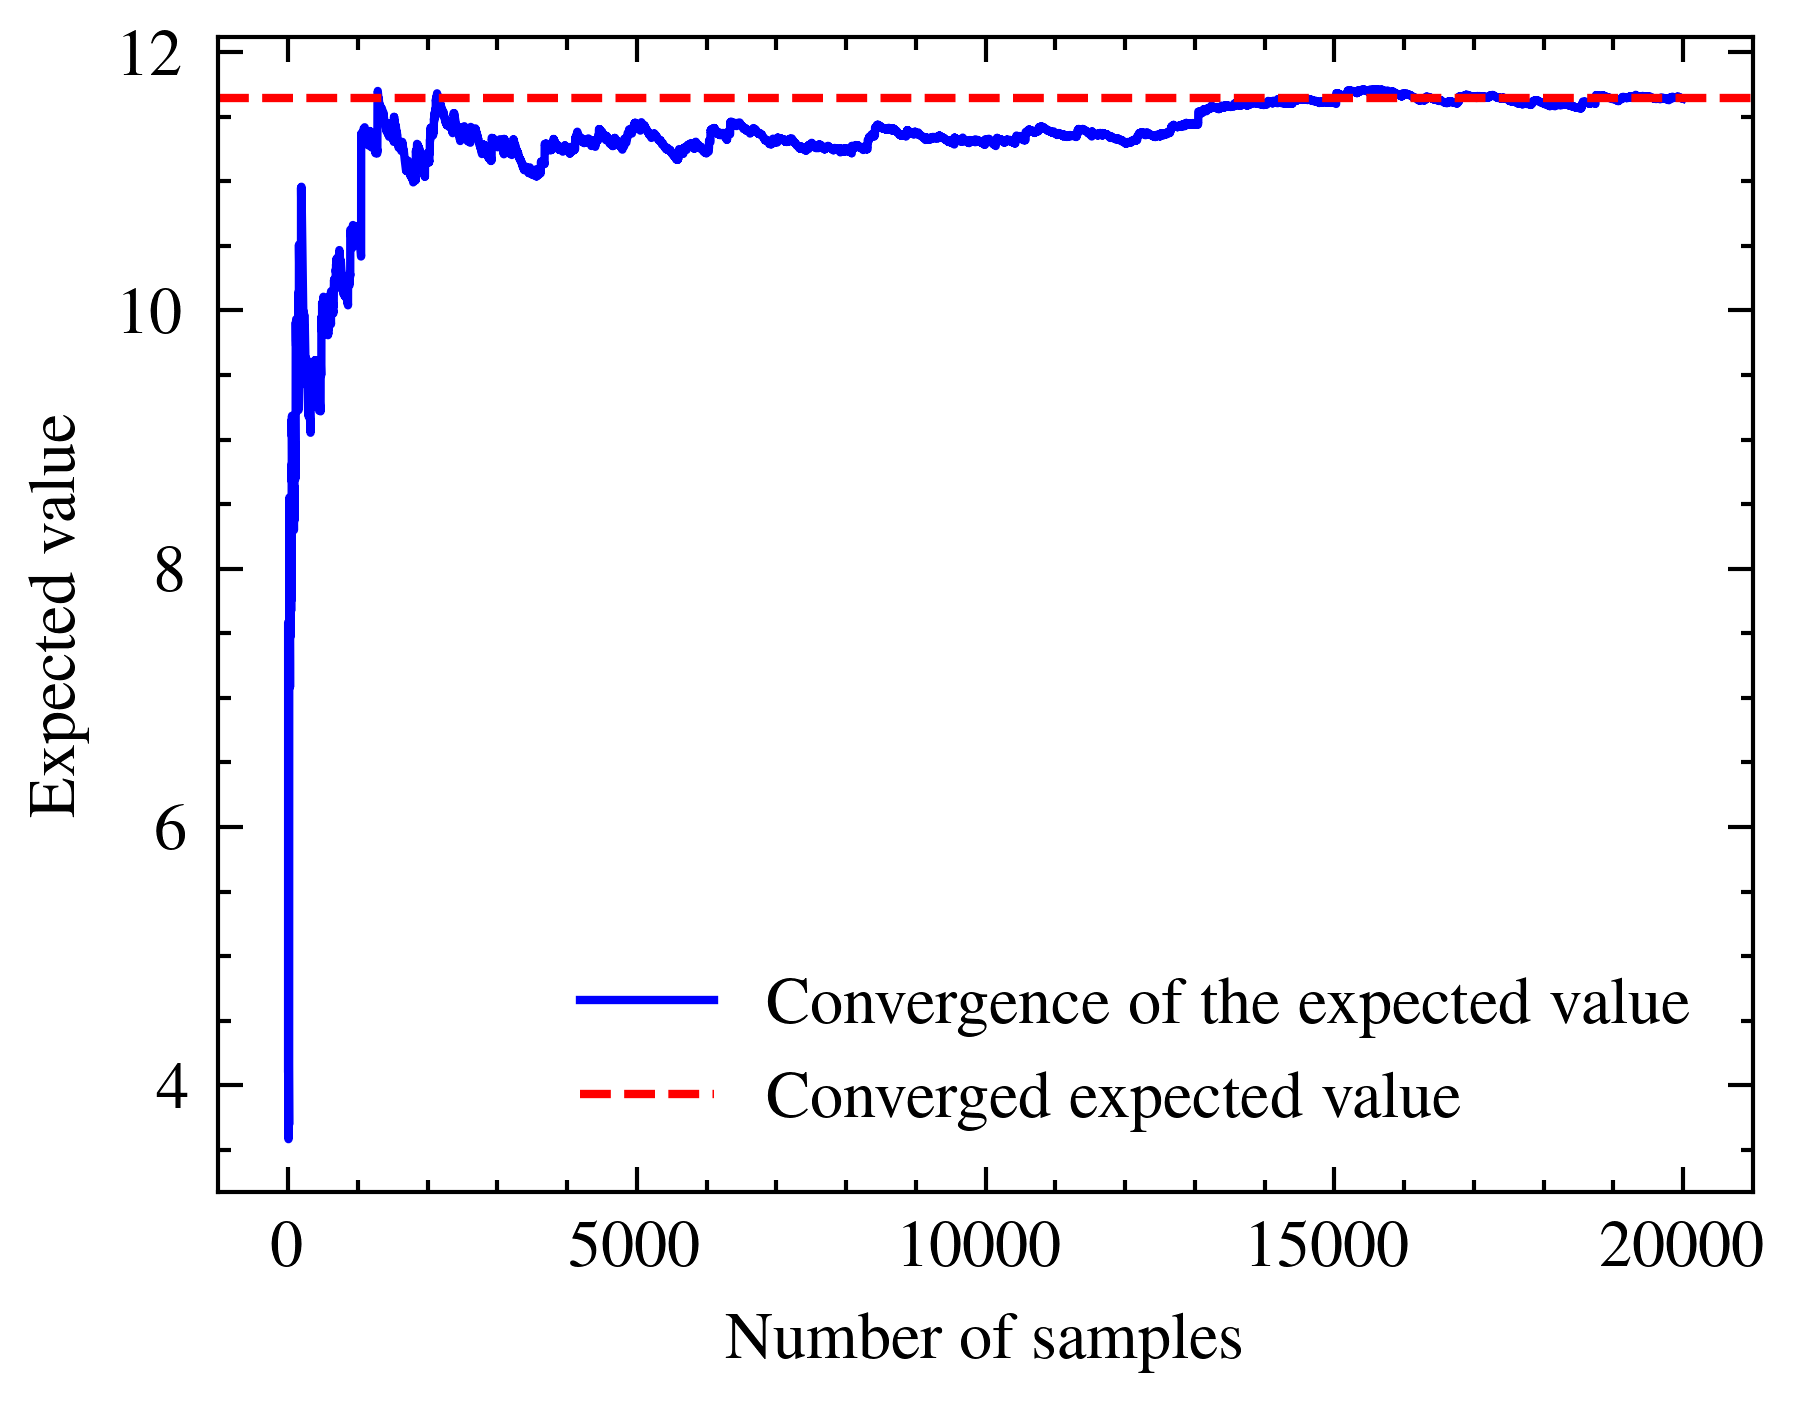
\includegraphics{imgs/convergence.png}
        \caption{Convergence of the Given Expectation Over 20,000 Iterations}
        \label{fig:convergence}
    \end{figure}
\end{frame}

\begin{frame}{Question 2}
    With $S_t$ as a Geometric Brownian Motion process, we have $S_t = S_0e^{(\sigma W_t + (r - \frac{\sigma^2}{2})t)}$ where $r = 0.05$, $\sigma = 0.20$, $S_0 = 90$, and $W_t$ is a standard Wiener process. We wish to estimate $\mathbb{E}(S_3)$.
\end{frame}

\begin{frame}{Question 2 Continued}

    \begin{itemize}
        \item We use a sufficiently large simulation size (20,000) to simulate $\mathbb{E}[S_3]$. The Wiener process is simulated using NumPy's
        builtin random number generator in the range $[0, \sqrt{t}]$, with $t = 3$.
        \item We calculate the expectation of $S_t$ by simply taking $\mathbb{E}[S_t] = S_0e^{rt}$.
    
    \end{itemize}

    \begin{tcolorbox}
        Simulated $\mathbb{E}[S_3]$ is $\boxed{104.2625934286796}$\\
        Expected $\mathbb{E}[S_3]$ is $\boxed{104.56508184554548}$
    \end{tcolorbox}
\end{frame}


\begin{frame}{Question 3}

    Our goal is to evaluate the following expected value and probability:
    \begin{itemize}
        \item $\mathbb{E}(X^{0.6}_{2})$
        \item $\mathbb{P}(X^{0.6}> 2)$
    \end{itemize}

    The Ito's processes $X$ evolve according to the following SDE:
    \begin{equation*}
        dX_t = \left( \frac{1}{4} + \frac{1}{3}X_t \right) dt + \frac{3}{5} dW_t, \quad X_0 = 2
    \end{equation*}
    where $W$ is a standard Wiener process.

\end{frame}


\begin{frame}{Question 3 Continued}
    \begin{itemize}
        \item We use a large sample size ($N = $ 1,000,000) with a time step of $2 / N = dt$ to simulate the process.
        \item We calculate the expected value of $X_{2}^{0.6}$ and the probability that $X_{2}^{0.6} > 2$.
    \end{itemize}
    We use the following algorithm to simulate the process:
    
    \begin{algorithmic}
        \For{$i = 1, 2, \ldots, N$}
            \State $dW = \sqrt{dt} Z_i$
            \State $X_{t_i} = X_{t_{i-1}} + \left( \frac{1}{4} + \frac{1}{3}X_{t_{i-1}} \right) dt + \frac{3}{5} dW$
            \State Update $W_{t_i} = W_{t_{i-1}} + dW$
        \EndFor
    \end{algorithmic}

    and calculate the expected value and probability using the simulated values.

\end{frame}

\begin{frame}{Question 3 Continued}
    The expectation and probability are calculated using the indicator function's sample mean.
    We do not have enough computing power to verify the results, but we conclude that $\mathbb{E}(X^{0.6}_2)$ has a {\color{red} minimum} value of $\approx 1.5$
    and is {\color{red} unbounded} above as $N \to \infty$. The probability that $X^{0.6} > 2$ varies $\in[0,1]$ according to the simulation's sample size, but 
    approaches $1$ as $N \to \infty$.
    
    We verify this graphically in the coming slides.
\end{frame}

\begin{frame}{Question 3 Continued}
    \begin{figure}
        \centering
        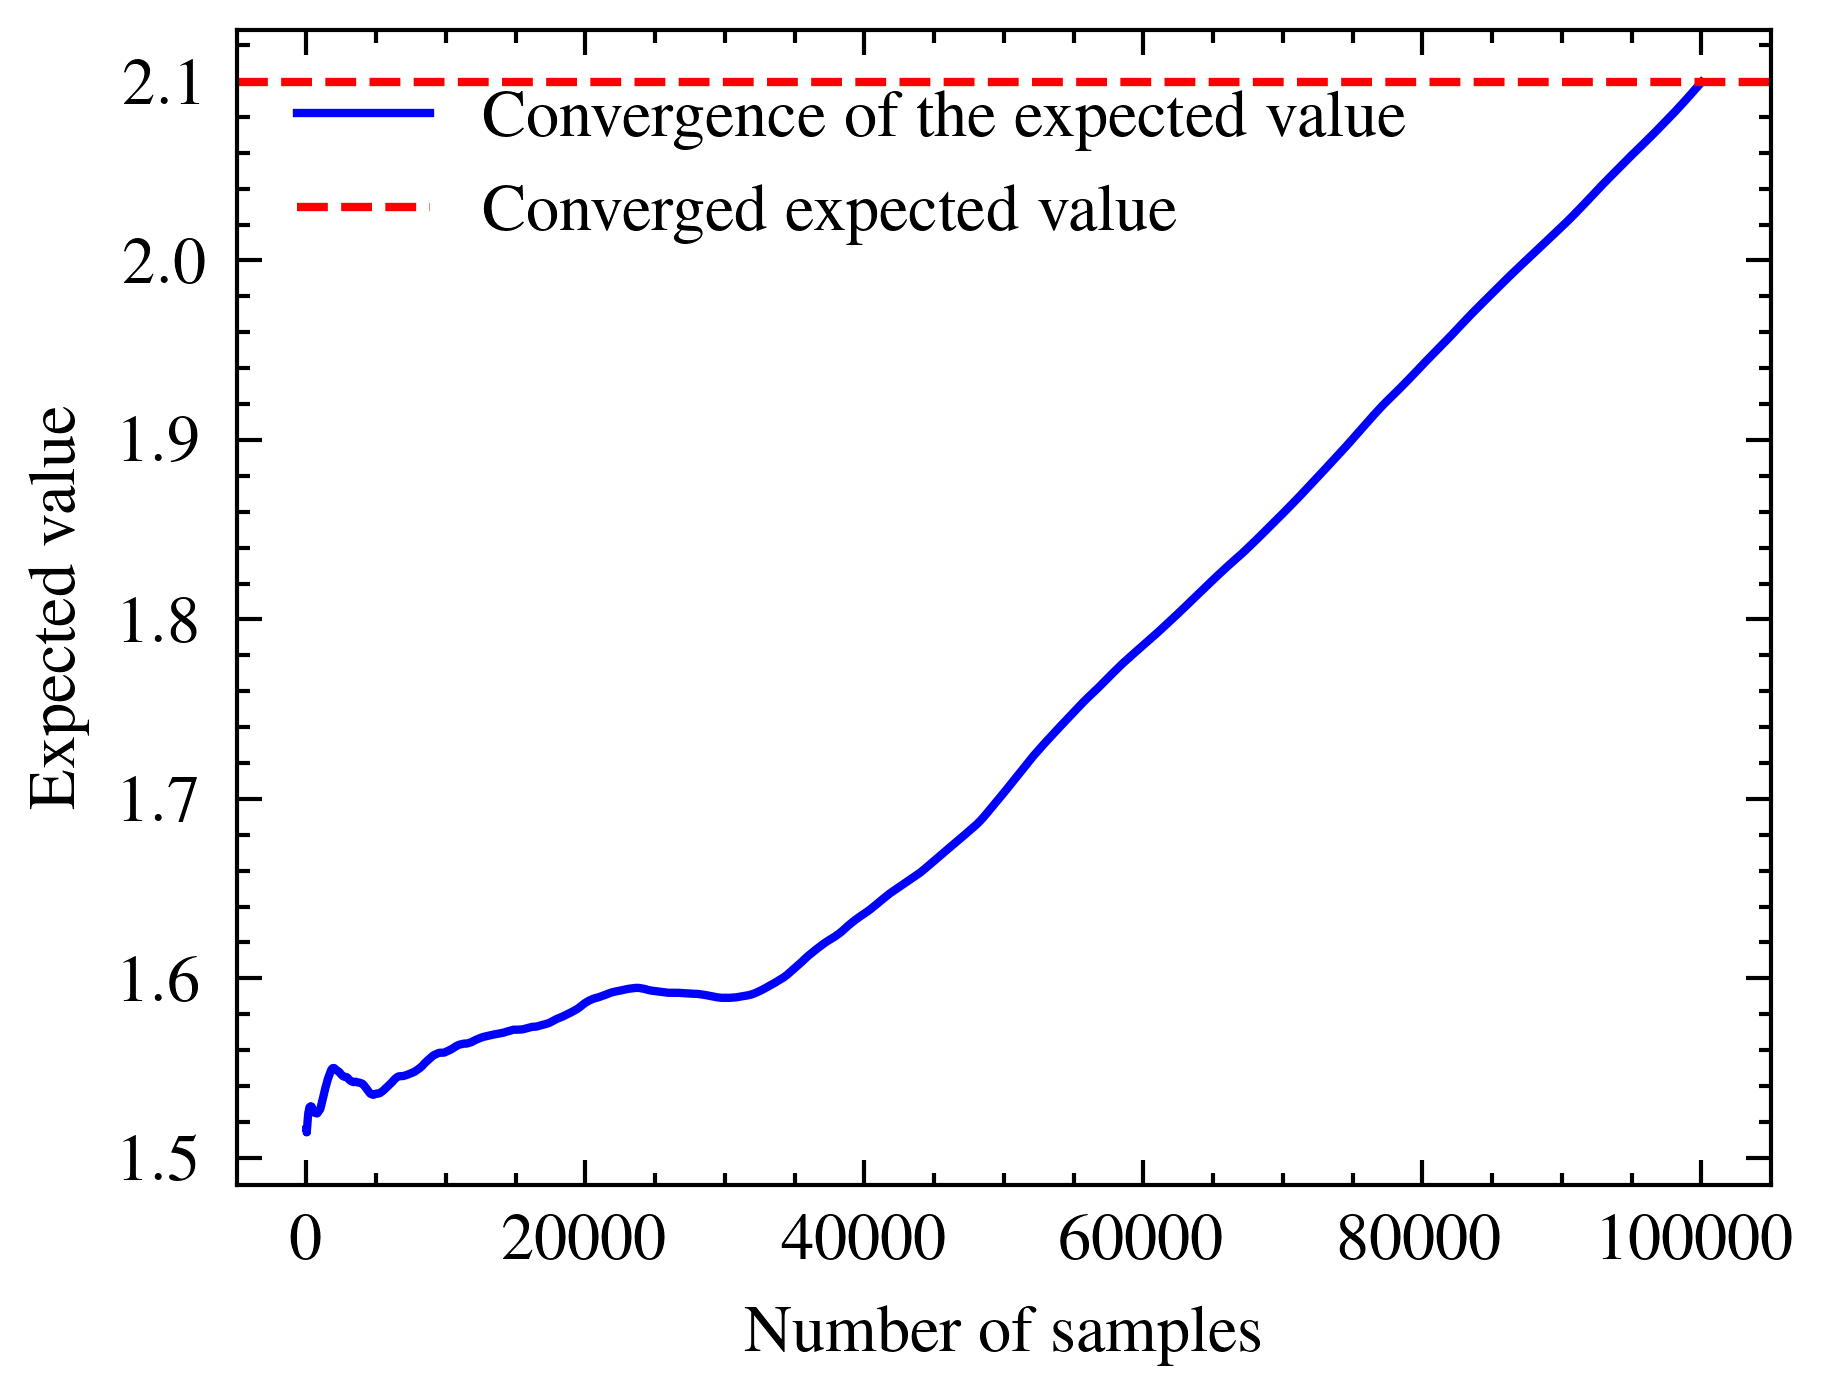
\includegraphics{imgs/convergence2.png}
        \caption{Convergence of the Expected Value and Probability Over 100,000 Iterations}
        % \label{fig:probability}
    \end{figure}

\end{frame}

\begin{frame}{Question 3 Continued}
    \begin{figure}
        \centering
        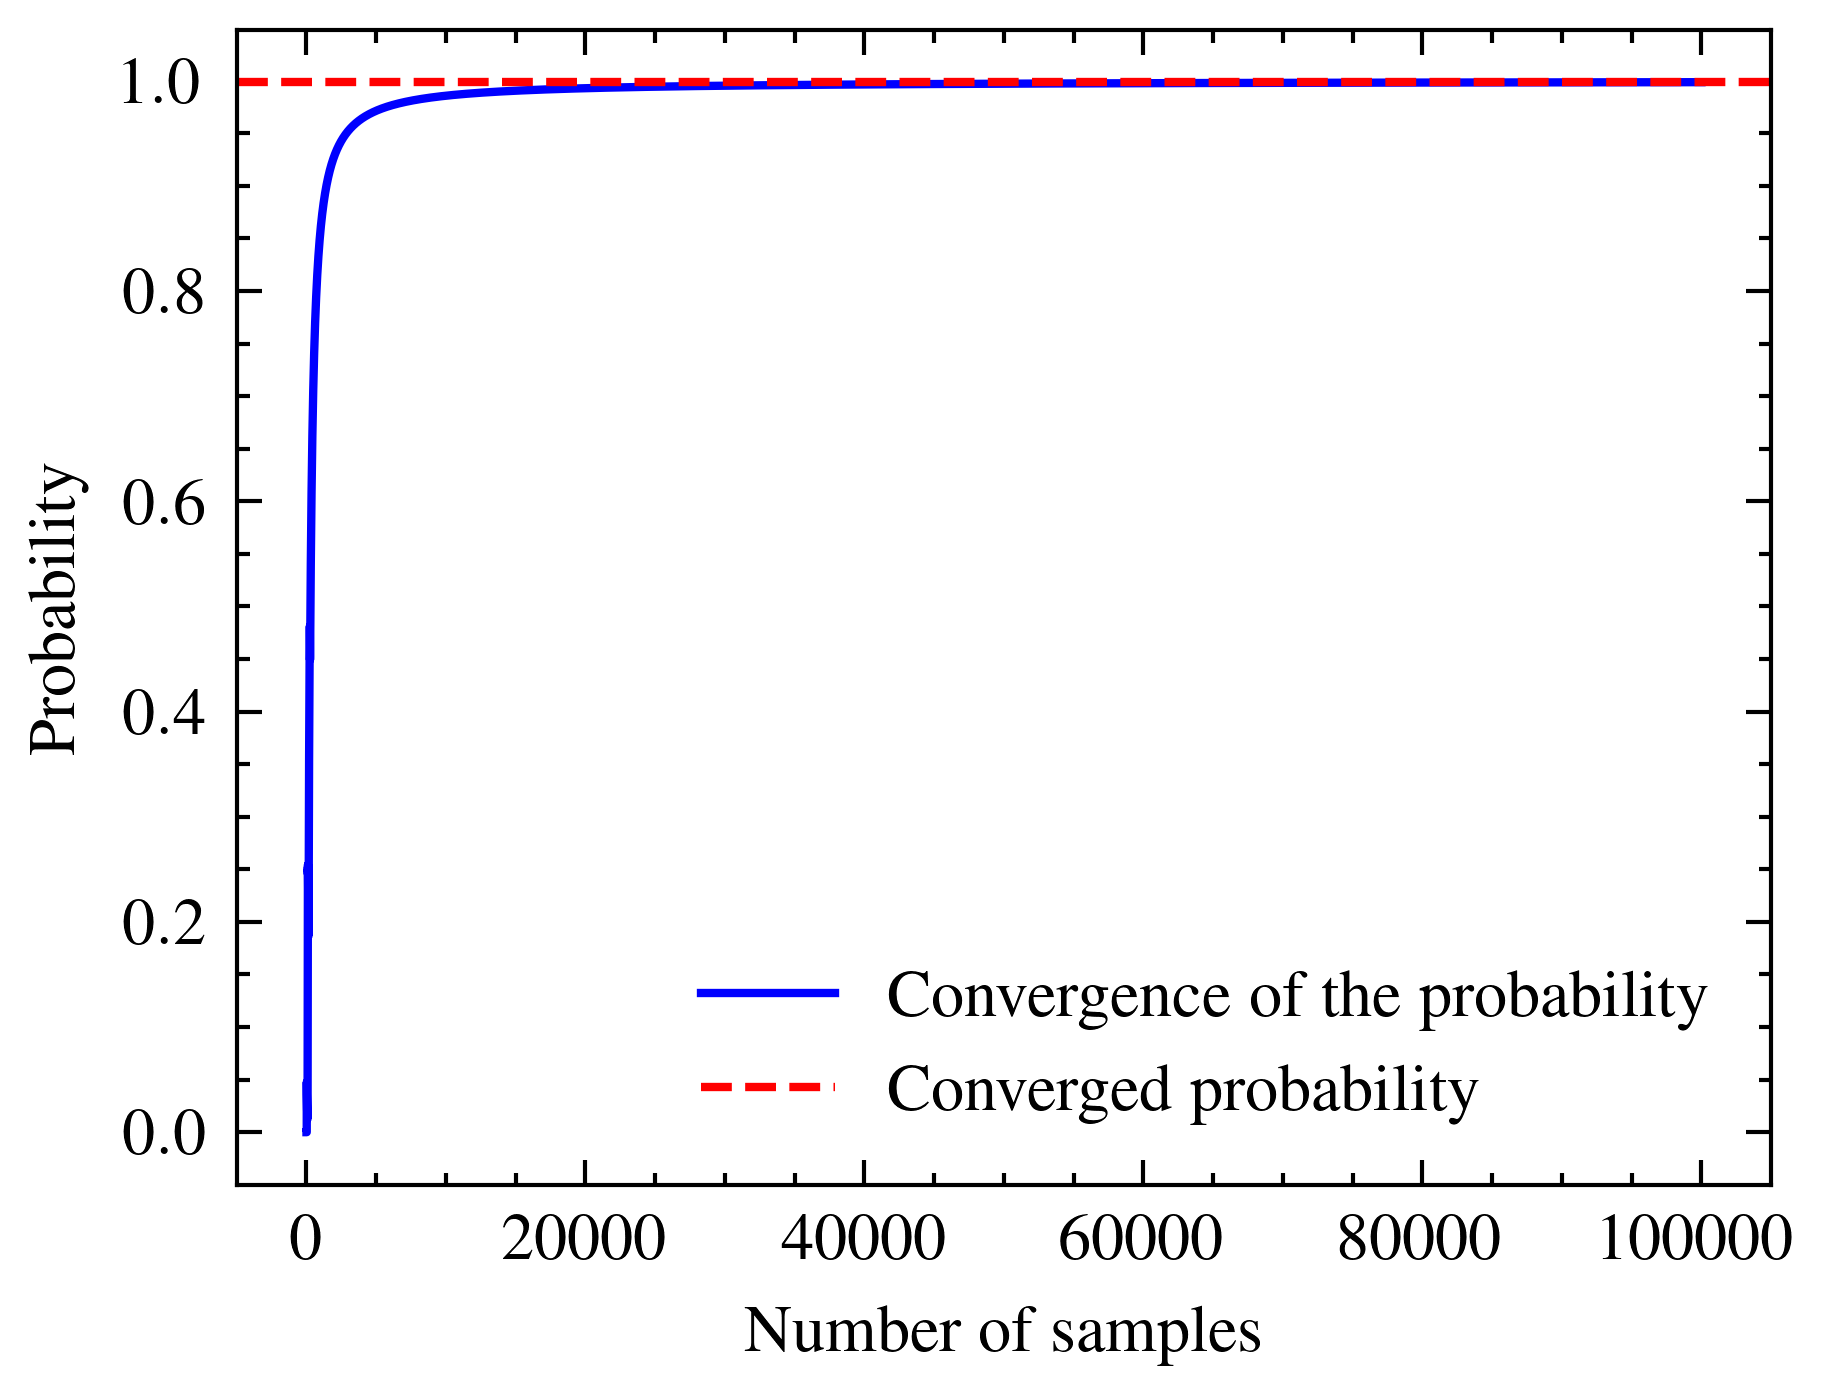
\includegraphics{imgs/probabilityconvergence.png}
        \caption{Convergence of the Probability Over 100,000 Iterations}
        % \label{fig:probability}
    \end{figure}

\end{frame}


\begin{frame}{Question 4}
    We consider the following SDE:
    \begin{equation*}
        dX_t = aX_t dt + bX_t dW_t, \quad X_0 = 100, \quad a = 0.07, \quad b = 0.12
    \end{equation*}

    \begin{itemize}
        \item We simulate this stochastic process using the discretization schemes of Euler-Maruyama.
        \item We compare the simulation with the analytical solution.
    \end{itemize}

    We use the following algorithm to simulate the process:
     
    \begin{algorithmic}
        \For{$i = 1, 2, \ldots, N$}
            \State $dW = \sqrt{dt} Z_i$
            \State $X_{t_i} = X_{t_{i-1}} + aX_{t_{i-1}} dt + bX_{t_{i-1}} dW$
            \State Update $W_{t_i} = W_{t_{i-1}} + dW$
        \EndFor
    \end{algorithmic}

    With the analytical solution given by $X_{\text{analytical}} = X_0 \exp((a - b^2/2)t + bW)$.
\end{frame}

\begin{frame}{Question 4 Continued}
    \begin{figure}
        \centering
        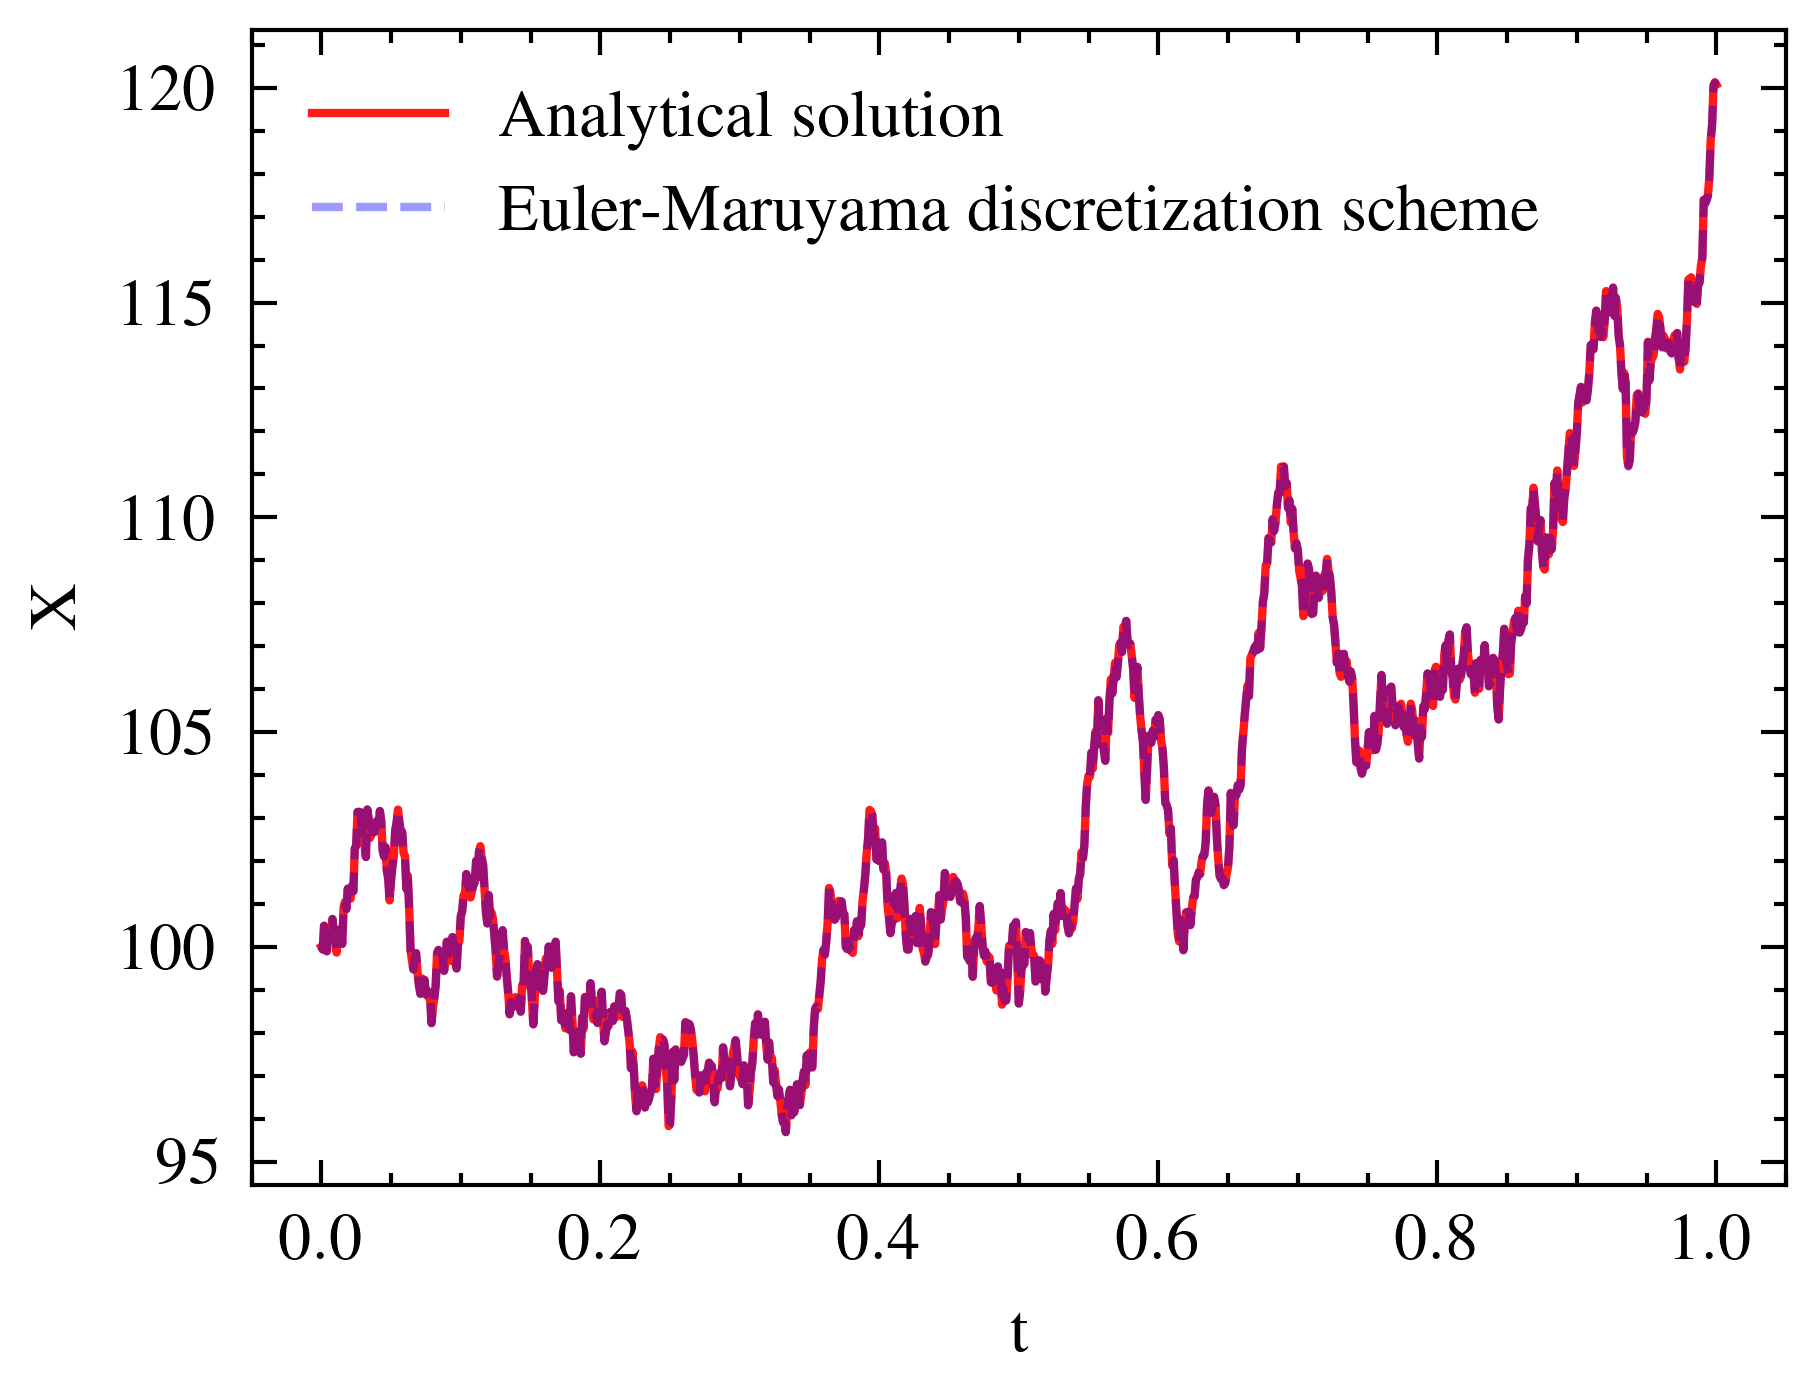
\includegraphics{imgs/eulermaruyama.png}
        \caption{Comparison of the Analytical Solution and the Euler-Maruyama Method}
        % \label{fig:question4}
    \end{figure}
\end{frame}

\begin{frame}{Question 4 Continued}
    We get a very close match between the analytical solution and the Euler-Maruyama method. The Euler-Maruyama method is a good approximation for the analytical solution.We calculate
    the sum of the absolute difference between the two methods and find that the average difference
    \begin{equation*}
        \text{Average Difference} = \frac{1}{N} \sum_{i=1}^{N} |X_{\text{analytical}} - X_{\text{Euler-Maruyama}}|
    \end{equation*}
    is $\approx 15.56230558918206$ and varies with the function.
\end{frame}

\begin{frame}{Question 4 Continued}
    \begin{figure}
        \centering
        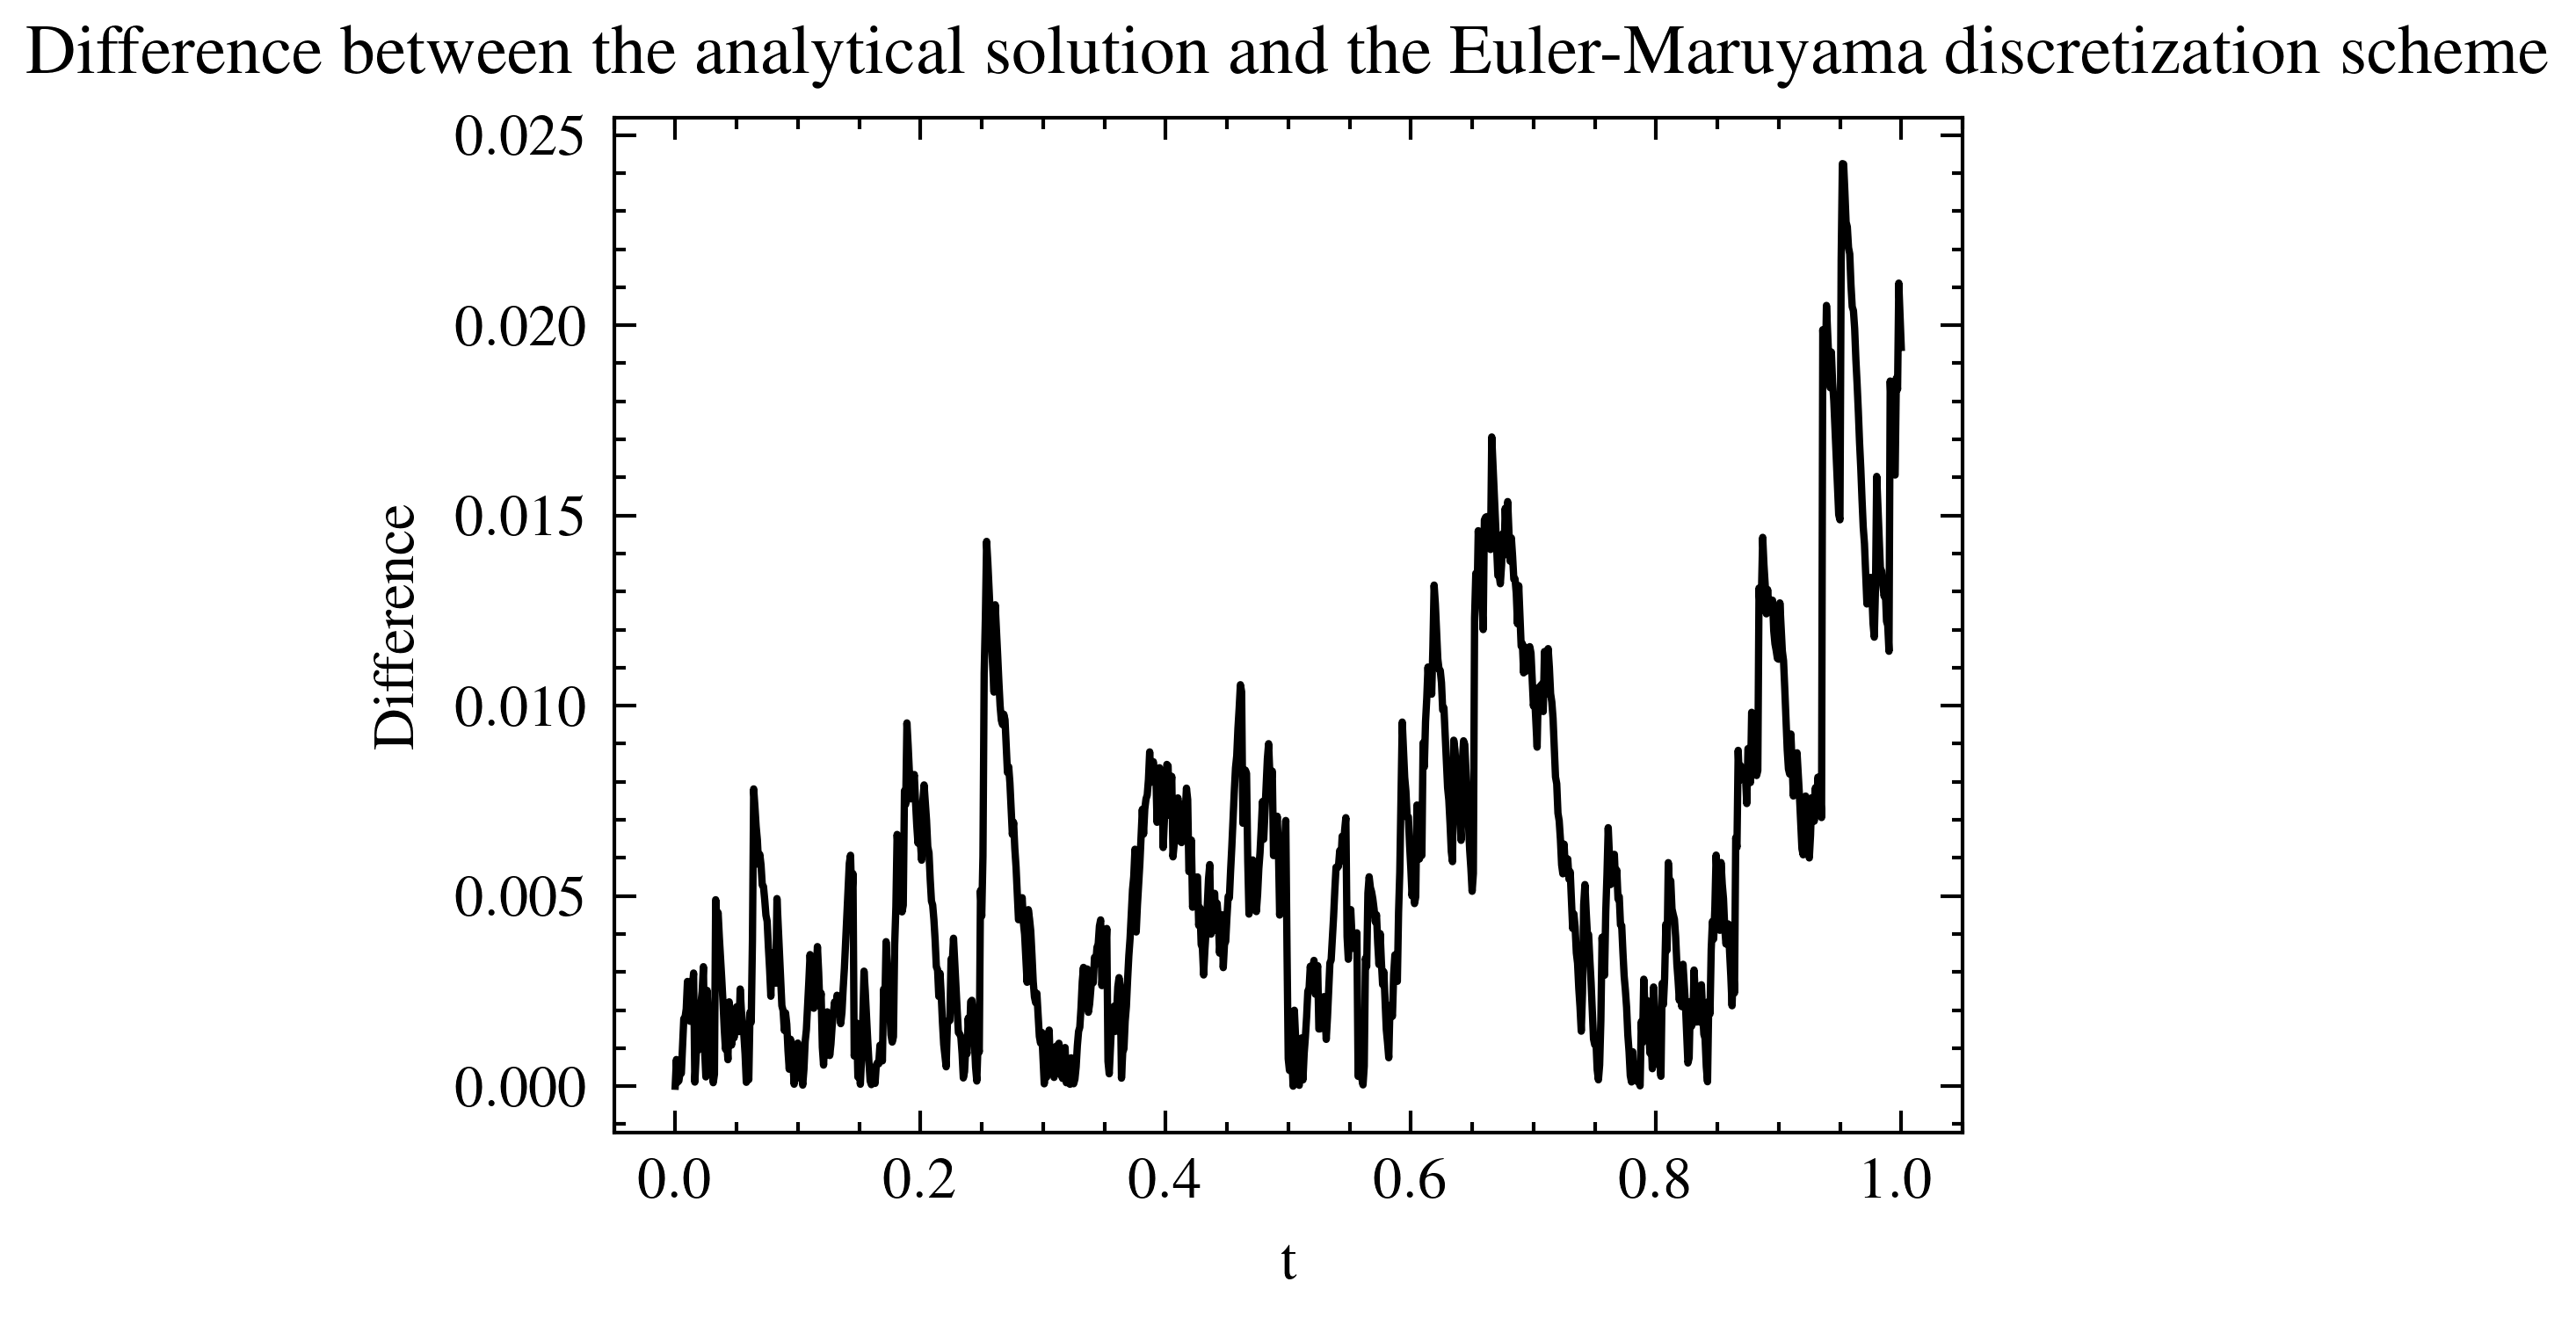
\includegraphics{imgs/difference.png}
        \caption{Difference Between the Analytical Solution and the Euler-Maruyama Method}
        % \label{fig:question4}
    \end{figure}
\end{frame}

\End
\begin{frame}[plain,standout]
      \centering
      Questions?
\end{frame}

\end{document}
